\documentclass{sig-alternate-2013}

% UTF8 support
\usepackage[utf8x]{inputenc}
\usepackage[T1]{fontenc}

\usepackage{graphicx}
\graphicspath{{figs/}}
\usepackage{tikz}
\usetikzlibrary{shapes}

\usepackage{array}

\usepackage{color, soul}

\newcommand{\eg}{{\textit{e.g.~}}}
\newcommand{\etal}{{\textit{et al.~}}}
\newcommand{\ie}{{\textit{i.e.~}}}

\usepackage[draft, nomargin, footnote]{fixme}

\begin{document}

\title{The Cognitive Correlates of Anthropomorphism}

\numberofauthors{2} 
\author{
\alignauthor
Séverin Lemaignan, Julia Fink, Pierre Dillenbourg\\
    \affaddr{Computer-Human Interaction in Learning and Instruction}\\
    \affaddr{Ecole Polytechnique Fédérale de Lausanne (EPFL)}\\
    \affaddr{CH-1015 Lausanne, Switzerland}\\
    \email{firstname.lastname@epfl.ch}
\alignauthor
Claire Braboszcz\\
    \affaddr{LabNIC}\\
    \affaddr{University of Geneva}\\
    \affaddr{\hl{CH-1015} Geneva, Switzerland}\\
    \email{claire.braboszcz@unige.ch}
}

\maketitle

\begin{abstract}

%Anthropomorphism in robotics is often discussed, and still appears to lack
%formal grounds. To tackle this issue, we recently proposed a first model of the
%dynamics of anthropomorphism, which reflects the evolution of anthropomorphism 
%over time, and accounts for non-monotonic effects like the so-called
%\emph{novelty effect}.
Based on our recently suggested model of the dynamics of anthropomorphism, we now
present initial ideas regarding the \emph{cognitive
correlates} induced by a sustained human-robot interaction. We
propose to distinguish three cognitive phases: (\emph{pre-cognitive},
\emph{familiarity}-based, and \emph{adapted}
anthropomorphism). We outline how these phases relate to the evolution of
anthropomorphism over time.

\end{abstract}

\section{Dynamics of Anthropomorphism}
\label{sec:dynamics_model}

Anthropomorphism refers to a \emph{social
phenomenon} that emerges from the \emph{interaction} between a robot and a
user. This includes for
instance people's tendency to ascribe emotional states, motivations or intentions to
a the robot~\cite{epley_when_2008}. As such, anthropomorphism is fundamentally dynamic.
We propose to understand "anthropomorphic effects" as observable manifestations of anthropomorphism.
Recently, we presented~\cite{lemaignan2014dynamics} a model of
anthropomorphism to formalize these dynamics.



%Many robotics researchers tend to believe that \emph{anthropomorphism}
%describes a static set of human-like features of a robot (like shape, speech
%capabilities, facial expression). We refer to these characteristics as the
%\emph{anthropomorphic design} of the robot~\cite{fink_anthropomorphism_2012}.
%\emph{Anthropomorphism}, on the other hand, 

Based on our own empirical research and theoretical work~\cite{fink_anthropomorphism_2012, fink_living_2013, fink2014which} 
%a literature review~\cite{fink_anthropomorphism_2012}, a long-term field study in a
%natural environment~\cite{fink_living_2013}, as well as two on-going child-robot
%experiments~\cite{fink2014which}, 
we believe that anthropomorphic effects do not
only evolve over time, but that they do so in non-monotonic ways, reflecting
cognitive processes experienced by the human peer. Before we suggest underlying cognitive correlates of different anthropomorphic effects, we first briefly review our recently proposed model of the dynamics of anthropomorphism~\cite{lemaignan2014dynamics}.
 
%Figure~\ref{fig:dynamics} shows our model of the long-term dynamics of
%anthropomorphic effects that
%we call the \emph{dynamics of anthropomorphism}~\cite{lemaignan2014dynamics}. By
%long-term interaction, we mean direct (non-mediated), repeated interaction with
%the same robot, over an extended period of time (longer than a week).
%
%In the next section, we suggest a cognitive interpretation of this model.
%
%\begin{figure}[htb]
%\centering
%
%
%\begin{tikzpicture}[scale=0.75]
%
%% background shading
%\path[fill=gray!20] (0,0) rectangle (0.6,5.5);
%\path[fill=gray!50] (0.6,0) rectangle (5.2,5.5);
%\path[fill=gray!20] (5.2,0) rectangle (9.8,5.5);
%\draw(0,5.5) node[anchor=south west] {\scriptsize \sc Initialization};
%\draw(4,5.5) node[anchor=south] {\scriptsize \sc Familiarization};
%\draw(7.5,5.5) node[anchor=south] {\scriptsize \sc Stabilization};
%% horizontal axis
%\draw[->] (0,0) -- (10,0) node[anchor=north] {$t$};
%\draw(5,-0.1) node[anchor=north] {\scriptsize Duration of interaction};
%
%
%% vertical axis
%\draw[->] (0,0) -- (0,6) node[anchor=east] {};
%\draw(-0.8,3) node[rotate=90,anchor=south] {\scriptsize Normalized level of anthropomorphic effects};
%
%\draw (-0.05, 3) -- (0.05, 3) node[anchor=east] {\scriptsize ICA$_{\mathcal B}$};
%\draw (-0.05, 4.1) -- (0.05, 4.1) node[anchor=east] {\scriptsize ICA$_{\mathcal A}$};
%\draw (-0.05, 0.6) -- (0.05, 0.6) node[anchor=east] {\scriptsize ICA$_{\mathcal C}$};
%
%% vertical axis - end
%\draw[->] (9.8,0) -- (9.8,2) node[anchor=east] {};
%\draw (9.8, 0.8) node[anchor=west] {\scriptsize SLA$_\mathcal{E}$};
%\draw (9.8, 1.4) node[anchor=west] {\scriptsize SLA$_\mathcal{D}$};
%\draw (9.8, .2) node[anchor=west] {\scriptsize SLA$_\mathcal{F}$};
%
%
%\draw[<-] (0.65,5) -- (0.8,5.2) node[anchor=east] {};
%\draw (0.9,5.3) node[anchor=west] {\tiny \it novelty effect};
%
%
%\draw[dotted] (0, 5) -- (6.2,5);
%\draw[dotted] (0, 3) -- (6.2,3);
%\draw[<->] (6.1,3) -- (6.1,5) node[anchor=east] {};
%\draw (6.2,4) node[rotate=90, anchor=north] {\tiny Expectation mismatch};
%
%\draw[<-] (1.7,4.4) -- (3.2,4.1) node[anchor=east] {};
%\draw[<-] (2.85,3.3) -- (3.2,4.1) node[anchor=east] {};
%\draw (3.2,4.1) node[anchor=west] {\tiny \it disruptive behaviors};
%%%%%%
%%% CURVES
%%%%%
%\begin{scope}[yscale=-1,shift={(-0.125,-0.4)}]
%
%% output of inkscape2tikz
%\path[draw=black]
%    (0.1250,-2.5620) .. controls (0.1451,-3.7193) and (0.4645,-4.5602) ..
%    (0.7044,-4.5633) .. controls (0.8413,-4.5633) and (0.9599,-4.5104) ..
%    (1.0794,-4.3971) .. controls (1.1989,-4.2841) and (1.3191,-4.1185) ..
%    (1.4588,-3.9181) .. controls (1.5287,-3.8183) and (1.5610,-4.1413) ..
%    (1.6381,-4.1420) .. controls (1.7378,-4.1420) and (1.6515,-3.6434) ..
%    (1.9554,-3.2280) .. controls (2.1466,-2.9667) and (2.3889,-2.7023) ..
%    (2.6819,-2.4292) .. controls (2.7551,-2.3607) and (2.7727,-2.8119) ..
%    (2.8771,-2.8180) .. controls (2.9742,-2.8180) and (2.9594,-2.2108) ..
%    (3.1665,-2.0209) .. controls (3.3340,-1.8673) and (3.5379,-1.7527) ..
%    (3.7508,-1.6236) .. controls (5.8366,-0.4852) and (8.0977,-0.2106) ..
%    (10.1250,-0.1860);
%\path[draw=black, dashed]
%    (0.1250,-3.6924) .. controls (0.1103,-4.0298) and (0.4645,-4.5602) .. 
%    (0.7044,-4.5633)
%    (3.7508,-1.6236) .. controls (4.9579,-0.9555) and (8.1358,-0.8261) .. 
%    (10.1250,-0.7946);
%\path[draw=black,dashed]
%    (0.1250,-0.1953) .. controls (0.1804,-3.3871) and (0.4645,-4.5602) .. 
%    (0.7044,-4.5633) .. controls (0.8413,-4.5633) and (0.9599,-4.5104) .. 
%    (1.0794,-4.3971)
%    (3.7508,-1.6236) .. controls (4.7654,-0.8505) and (6.5955,0.3538) .. 
%    (10.1250,0.4062);
%
%\end{scope}
%
%\end{tikzpicture}
%
%\caption{Dynamics of anthropomorphism. Different levels of anthropomorphic effects
%are observable based on the duration of an interaction between a human user and a robot.
%The non-monotonic curve of anthropomorphic effects merges in three phases:
%initialization, familiarization, and stabilization.}
%
%\label{fig:dynamics}
%\end{figure}

%We distinguish three main phases:
%\emph{initialization}, \emph{familiarization} and \emph{stabilization},
%preceded by a \emph{pre-interaction} phase. In the pre-interaction phase,
%users build an \emph{initial capital of anthropomorphism} (ICA). Once the
%interaction starts, the level of anthropomorphism increases due to the
%\emph{novelty effect}~\cite{kanda_interactive_2004}, and then decreases to
%reach a \emph{stabilized level of anthropomorphism} (SLA).  During the
%interaction, unpredicted behaviors of the robot (\emph{disruptive behaviors})
%may lead to local increase of the level of anthropomorphism.

%\subsection*{Three phases}
%\label{sec:phases}

Our model of the dynamics of anthropomorphism tries to formally describe a curve that
represents the level of anthropomorphic effects which can be observed in a long-term human-robot interaction. By long-term interaction, we mean direct (non-mediated), repeated interaction with the same robot, over an extended period of time (longer than a week).
The level of anthropomorphic effects evolves in a non-monotonic way and merges in three phases: initialization, familiarization, and stabilization.

%We distinguish three main phases, depicted in different shades in
%Figure~\ref{fig:dynamics}.

\paragraph*{Initialization}
During this first short phase, \emph{initialization}, which lasts from a couple
of seconds to a couple of hours, an increased level of
anthropomorphism can be observed. In the very beginning, the \emph{initial capital of anthropomorphism (ICA)} indicates the likelihood of anthropomorphism in a human-robot interaction.
This value can be understood as the user's initial expectations toward the robot,
and is composed of three main factors: personality of the human, design of the
robot, and context/purpose of the interaction. 
%The variability of this value is pictured in Figure~\ref{fig:dynamics}). 
The end of the initialization phase is typically
characterized by a peak of anthropomorphic manifestations that corresponds to the maximum of the \emph{novelty effect}.

\paragraph*{Familiarization}
The following phase, \emph{familiarization}, lasts longer (up to several days) and
models the process of the human getting acquainted to the robot: by observation
and interaction, the human builds a model of the robot's behavior that allows
him/her to predict the robot's actions. We observe a decrease of
anthropomorphic effects during this phase, that we explain by the acquired
ability to predict the behavior of the robot: the initial apparent behavioral
complexity vanishes, and the robot is considered more and more as a tool.

\paragraph*{Stabilization}
During the \emph{stabilization} phase the level of anthropomorphic effects tends to
stabilize over a longer period of time, to reach a \emph{stabilized
level of anthropomorphism (SLA)}. The SLA may be zero (no anthropomorphic
effects observed anymore), but it may also remain at a higher level. Like the
ICA, the SLA is a multi-factor value that depends on the human, the robot and
the interaction context.

\section{Cognitive interpretation}
\label{sec:cognitivemodel}

The proposed cognitive correlates of anthropomorphism, and how they relate to the just described dynamics, are based on existing explanations of anthropomorphism. 

\paragraph*{Explanations for anthropomorphism}

%Anthropomorphism represents just one of many examples of induction whereby
%``people reason about an unknown stimulus based on a better-known representation
%of a related stimulus"~\cite{epley_when_2008}, in this case reasoning about a
%non-human agent based on representation of the self or other humans.

According to Lee \textit{et al.} \cite{lee_human_2005},
there are two main perspectives in explaining people's tendency to
anthropomorphize. First one explains anthropomorphism from the design of
the artifact. It assumes that humans
directly respond to life-like or social cues that an object or system emits,
without thoughtful mental processing, by simply applying stereotypes and
heuristics to it. 
%In fact, from early childhood on, humans are inherently
%well-trained to perceive life \cite{epley_seeing_2007}. 
%Schmitz~\cite{schmitz_concepts_2011} describes that within the visual scope of design,
%the outer appearance can have an important impact on the overall perception of
%an object.
The basic assumption is that if an artifact appears much like a
human, it is likely to be treated similar to a human. If this explanation of
anthropomorphism is correct, people may respond automatically to social cues
emitted by a robot, and apply human-human social schemas and norms to these
interactions.

The second perspective applies a human-centered, cognitive viewpoint where
anthropomorphism is described through people's specific mental model they
construct about how an artifact works the way it does.
We then anthropomorphize because it allows us to
explain things we do not understand in terms that we do understand, and what
we
 understand best is ourselves as human
beings~\cite{hegel_understanding_2008}. This is consistent with the
\emph{familiarity thesis} which claims that we
understand the world
 based upon a mental model of the world that we are most
familiar with.
% Consequently, people tend to thoughtfully develop a mental
%model of agents in
% their environment and make inferences about it based on
%what is familiar to
% them.
 This point of view implicitly builds on a person's
ability to attribute
 mental states to oneself and others (\ie the availability
of a \emph{theory of
 mind}~\cite{premack1978does}). 
 
% A theory of  mind for other
%agents enables us to
% attribute intentionality to those agents
%\cite{leslie_pretense_1987,admoni_multi-category_2012}. Previous research
%examined the validity of the mental model concept with various kinds of robots
%\cite{schmitz_concepts_2011,kiesler_mental_2002}. Findings suggest that people
%tend to hold richer mental models about anthropomorphic robots in contrast to
%mechanic ones \cite{kiesler_mental_2002}.


\begin{figure}[htb]
\centering
%\resizebox{\linewidth}{!}{
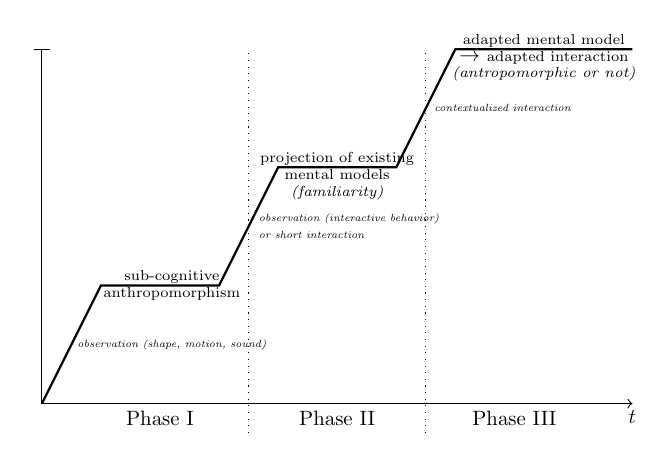
\begin{tikzpicture}[scale=0.75, transform shape]
\baselineskip=8pt

% horizontal axis
\draw[->] (0,0) -- (10,0) node[anchor=north] {$t$};
% labels
\draw   (2,0) node[anchor=north] {Phase I}
        (5,0) node[anchor=north] {Phase II}
        (8,0) node[anchor=north] {Phase III};

\draw[dotted] (3.5, -0.5) -- (3.5,6);
\draw[dotted] (6.5, -0.5) -- (6.5,6);

% vertical axis
\draw[-|] (0,0) -- (0,6) node[anchor=east] {};
% Us
\draw[thick] (0,0) -- (1,2) -- (3,2) -- (4,4) -- (6,4) -- (7,6) -- (10,6);

\draw (2.2,2) node[align=center] {\scriptsize{sub-cognitive}\\\scriptsize{anthropomorphism}}; %label
\draw (5,3.85) node[align=center] {\scriptsize{projection of existing}\\\scriptsize{mental models}\\\scriptsize{\it (familiarity)}}; %label
\draw (8.5,5.85) node[align=center] {\scriptsize{adapted mental model} \\ $\to$ \scriptsize{adapted interaction}\\\scriptsize{\it (antropomorphic or not)}}; %label

\draw (2.2,1) node[align=left] {\tiny{\it observation (shape, motion, sound)}}; %label
\draw (5.2,3) node[align=left] {\tiny \it observation (interactive behavior) \\ \tiny \it or short interaction}; %label
\draw (7.8,5) node[align=left] {\tiny \it contextualized interaction}; %label

\end{tikzpicture}
%}
\caption{The three cognitive phases of anthropomorphism: Phase I is the instinctive,
sub-cognitive identification of living peers. {\it Empathy} is characteristic
of this stage. After longer observation or short, non-contextualized interaction
(typically, a lab environment), the user enters Phase II: the user projects a
mental model he/she is already familiar with onto the robot. After longer {\it
contextualized} interaction (typically, at home), the user enters Phase III of
anthropomorphism: the user recomposes an accurate mental model of the robot,
based on experience. This leads to adapted interaction modalities, that may
still be anthropomorphic, or not.}
\label{fig:cognitivemodel}
\end{figure}

\paragraph*{Cognitive Processes and Phases}

The main underlying cognitive process in anthropomorphism is understood as
perceiving and reasoning about something non-human and unfamiliar based on
one's representation of the familiar and well-known concept of being
human~\cite{epley_when_2008}. This led us to interpret the phases of
anthropomorphic interactions as parallel cognitive phases.

The so-called \emph{phase I} is the instinctive, pre-cognitive identification
of living peers. This is supported by studies done by Rosenthal-von der Pütten
\textit{et al.}~\cite{rosenthal-vonderputten_experimental_2013} who
investigated the neural correlates of emotional reactions of humans towards a
robot. {\it Empathy} is characteristic of this stage.

After a longer observation period (typically including complete action
sequences of the robot) or short interaction (touching, short talk like
greetings), we suggest the human enters the cognitive \emph{phase II}: in this
phase, the human starts building a behavioral and cognitive model of the robot
that would support both the observed and imagined capabilities of the robot.
The \emph{familiarity thesis}~\cite{hegel_understanding_2008} would support the
idea that the human first projects onto the robot mental models of similar
agents he/she is already familiar with (ranging from animals to human adults,
to pets and children).

The cognitive \emph{phase III} occurs after a \emph{contextualized}
interaction. A \emph{contextualized} interaction is \emph{explicitly
purposeful} (the purpose of the interaction, be it purely entertainment, is
explicit and conscious to the human), and takes place in an environment that
fosters a stronger cognitive (and possibly affective/social) commitment from
the human in the interaction (typically, at home). During this interaction, the
human iteratively restates and reshapes his/her behavioral and mental model of
the robot (\emph{How does the robot react to such and such situation/input?
What does the robot know about me? About our environment? What
can the robot learn?}, etc.).

This mental process heavily depends on the human understanding of the robot's
inner working, as well as his/her own tendency to anthropomorphize, but at this
stage, the \emph{perception} of the robot (its shape for instance) and its
intended \emph{purpose} play a less important role. It is mostly a
human-centric process.  The result of this third phase would be an iteratively
adapted cognitive model of the robot.

\paragraph{Relation to the model of anthropomorphism} 

These cognitive phases overlap but do not exactly match the
\emph{Initialization}, \emph{Familiarization} and \emph{Stabilization} phases
introduced in our model of the dynamics of anthropomorphism, and we are currently
investigating the relations between both. In particular, cognitive phases I and
II are both included in the \emph{initialization} phase of the anthropomorphism
model.

Sub-cognitive anthropomorphism typically \emph{initiates} the novelty effect by
rapidly engaging the human in the interaction through an initial projected
\emph{agency}, whereas cognitive phase II (projection of familiar mental
models) supports the novelty effect by inducing beliefs that the robot is set
up with possibly complex cognitive abilities.

The cognitive phase II also overlaps with the \emph{familiarization} phase: as
(s)he get used to the robot, we hypothesize the human restates and adapts its
cognitive model of the robot by iteratively reshaping pre-existent, familiar
models until it provides a satisfying support to explain and justify the
observed robot behavior.

A \emph{stable level of anthropomorphism} is reached when the adaptation
process depicted in cognitive phase III reached a stable state, \ie the human
experience with the robot is correctly supported by the cognitive model the
human has built.

\section{Conclusion}
\label{sec:conclusion}

This discussion on the cognitive correlates of the dynamics
of anthropomorphism are speculative, and only indirectly supported by
experimental evidence. New experiences need to be designed to specifically test
these hypothesis.\fxnote{...}


Anthropomorphism is traditionally understood as the interactions between the
anthropomorphic design of a robot and the psychological determinants of the
user. We have found out that the duration and context of the interaction is a
third factor that plays a key role. In this preliminary report, we sketch a new
formal model of anthropomorphism that accounts for these three factors and also
explicits the dynamics of anthropomorphism. We introduce the concepts of
\emph{initial capital} and \emph{stabilized level of anthropomorphism} as
compound factors to characterize the profile of a given anthropomorphic
interaction.

While not definitive, we hope that this contribution may ultimately consolidate
the scientific grounds of anthropomorphism, and provides support for further
research on long-term acceptance of robots in human environments.

We hope that it may support further
discussions and reflections on how anthropomorphism impacts human-robot
interaction on the long run, and also foster research on the affective bonds
induced by anthropomorphic projections on robots.


\bibliographystyle{IEEEtran}
\bibliography{biblio} 
\end{document}
